\documentclass[tikz,border=5pt]{standalone}
\usepackage{tikz}
\usetikzlibrary{arrows.meta}
\definecolor{nebula}{HTML}{6366F1}
\definecolor{spark}{HTML}{14B8A6}
\definecolor{ink}{HTML}{334155}
\begin{document}
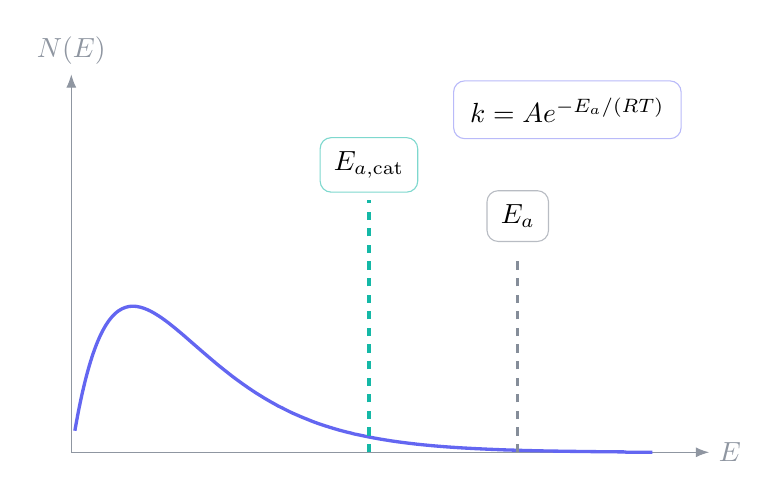
\begin{tikzpicture}[font=\sffamily,>=Latex,x=.9cm,y=1cm]
  \draw[->,ink!55] (0,0)--(9,0) node[right] {$E$};
  \draw[->,ink!55] (0,0)--(0,4.8) node[above] {$N(E)$};
  \draw[very thick,nebula,domain=.05:8.2,samples=160,smooth]
    plot(\x,{5.8*\x*exp(-1.15*\x)});
  \draw[dashed,very thick,spark] (4.2,0)--(4.2,3.2);
  \draw[dashed,very thick,ink!60] (6.3,0)--(6.3,2.5);
  \node[draw=spark!55,rounded corners=4pt,fill=white,inner sep=5pt] at (4.2,3.65) {$E_{a,\mathrm{cat}}$};
  \node[draw=ink!35,rounded corners=4pt,fill=white,inner sep=5pt] at (6.3,3.0) {$E_a$};
  \node[draw=nebula!45,rounded corners=4pt,fill=white,inner sep=6pt] at (7.0,4.35)
    {$k=Ae^{-E_a/(RT)}$};
\end{tikzpicture}
\end{document}
